	%====================================================================================================
	% ?????
	%====================================================================================================
	% TCC
	%----------------------------------------------------------------------------------------------------
	% Autor				: Jasane Schio
	% Orientador		: Gedson Faria
	% Co-Orientador		: Angelo Darcy
	% Instituição 		: UFMS - Universidade Federal do Mato Grosso do Sul
	% Departamento		: CPCX - Sistema de Informação
	%----------------------------------------------------------------------------------------------------
	% Data de criação	: 01 de Outubro de 2015
	%====================================================================================================
	
	\definecolor{dkgreen}{rgb}{0,0.6,0}
	\definecolor{gray}{rgb}{0.5,0.5,0.5}
	\definecolor{mauve}{rgb}{0.58,0,0.82}
	
	\lstset{frame=tb,
		language=C++,
		aboveskip=3mm,
		belowskip=3mm,
		showstringspaces=false,
		columns=flexible,
		basicstyle={\small\ttfamily},
		numbers=none,
		numberstyle=\tiny\color{gray},
		keywordstyle=\color{blue},
		commentstyle=\color{dkgreen},
		stringstyle=\color{mauve},
		breaklines=true,
		breakatwhitespace=true,
		tabsize=3
	}
	\chapter{Metodologia e Desenvolvimento} \label{Cap:Processamento}
	
			Para o desenvolvimento foi escolhida a biblioteca OpenCV por ser OpenSource, multiplataforma, uma grande quantidade de métodos e algoritmos já implementados	e pelo seu rápido desempenho de máquina.
			A linguagem escolhida para o desenvolvimento foi o C++ pois é uma linguagem de programação compilada, o que torna sua execução mais rápida que as linguagem interpretadas, tendo assim grande desempenho e por ser uma linguagem orientada objeto. 
			
			O sistema desenvolvido é separado em duas partes: Processamento e Interface Gráfica.
			A parte de Processamento é onde são feitas as partes de aquisição de imagem, processamento de imagem, conversão de imagem para modelo de cor HSV, seleção de pontos de cor e contagem de ocorrência de cor. Já a interface gráfica, é a onde ocorre a entrada do usuário para assim ser feita a calibração manual de mínimos e máximos de cada cor.
		
	
	Passos do projeto:
	\begin{description}
		\item[Aquisição de imagens em vídeo:] Nesse passo as imagem são adquiridas via câmera USB.
		
		\item[Identificação de Objetos:]
				 Durante o processo de aquisição de imagem são selecionados os objetos, quais serão usados como base para a detecção de máximos e mínimos de cores.
		\item [Cálculo de Mínimos e Máximos:]
		 Nessa etapa são levados em consideração os objetos teste. A imagem é "varrida"  por pixel na localidade dos objetos-teste e assim são salvos seus valores e feito a contagem de ocorrências de cada cor.		
	\end{description}


	\section{Projeto}
	\subsection{Organização do Projeto}
	 O projeto foi desenvolvido seguindo o paradigma de programação conhecido como  Orientação à Objetos, esse paradigma baseia-se na utilizaç~ao de objetos individuais para criaçao de um sistema maior e complexo. A IDE usada para o desenvolvimento foi a QT Creator. Esta separada o projeto em três pastas, Headers, Sources e Forms. Na pasta Headers estão os arquivos de cabeçalho(.h) onde estão as declarações dos métodos e variáveis usados nas classes  executáveis. Já na pasta Sources estão os arquivos fonte(.cpp), são nesses arquivos que os métodos declarados nos arquivos da pasta Header são implementados. Na pasta Forms está o arquivo de interface gráfica(.ui) que é usado no projeto para ser a ponte entre o usuario e as funções do sistema.
	 
	\begin{figure}[!h]
		\centering
		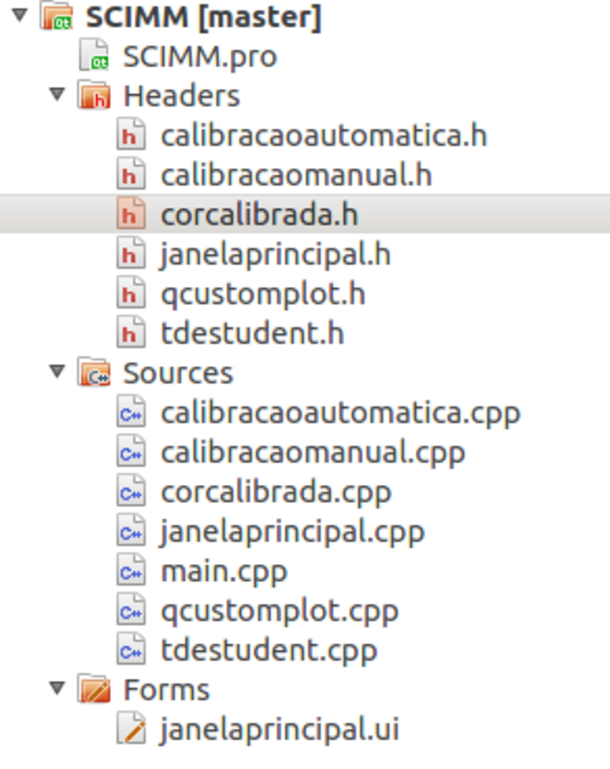
\includegraphics[width=0.2\textwidth]{organizacaoProjeto.pdf}
		\caption{Organização das pastas do projeto}
		\label{Organizacao do Projeto}
	\end{figure}
	Cada arquivo de cabeçalho possui um arquivo fonte correspondente, formando assim uma Classe, com exceção do arquivo fonte main, pois para este arquivo não há a necessidade.
	As classes desenvolvidas no projeto são:
 calibracao, manual, automatica, corcalibrada, janelaprincipal e tdestudent. Já a classe qcustomplot é um componente para auxilio em plotagem de gráficos e vizualização de dados\cite{QCustomPlot}.
Para melhor entendimento da interação entre as classes a figura 3.2 trás o diagrama de classes do projeto.
	 \begin{figure}[!h]
	 	\centering
	 	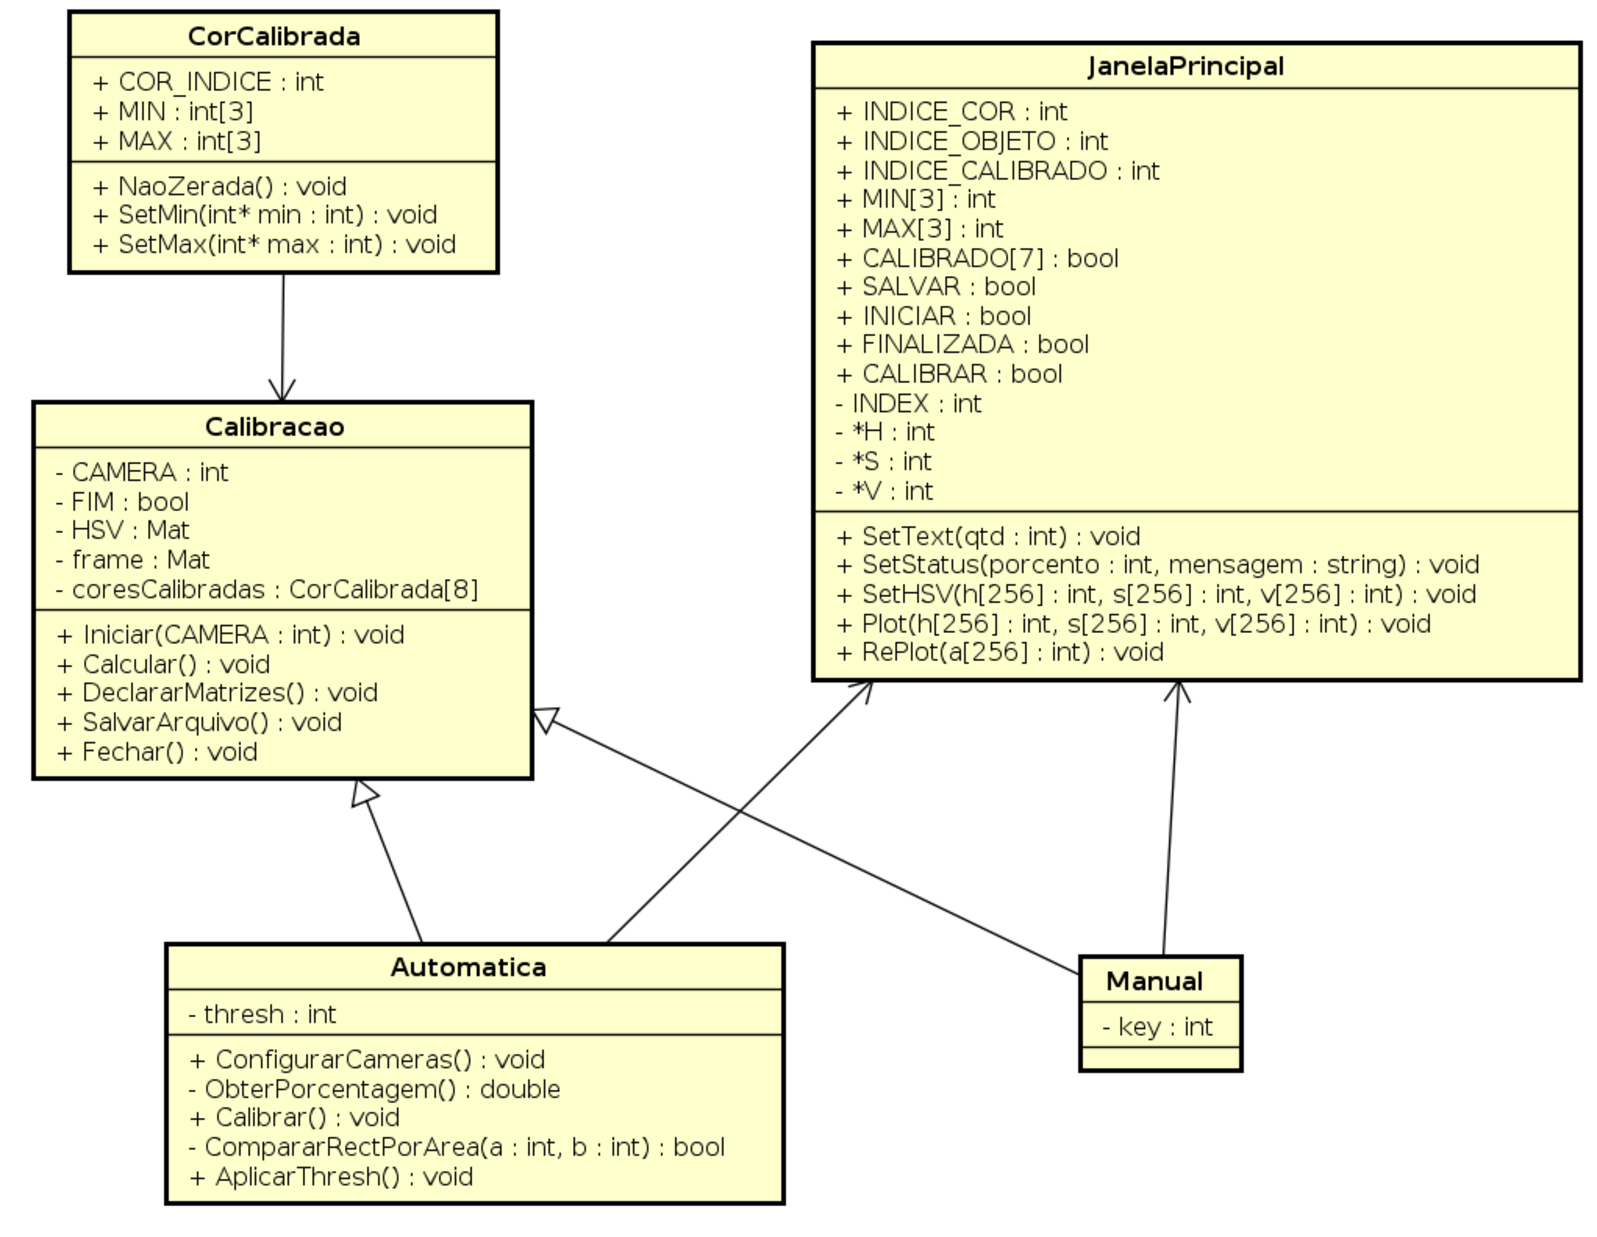
\includegraphics[width=0.8\textwidth]{diagramadeclasse.pdf}
	 	\caption{Diagrama de Classes do projeto}
	 	\label{DiagramaDeClasse}
	 \end{figure}\newpage


\subsection{Classes}
	\begin{description}

	\item [main] esta é a classe executavel do sistema, ela inicia o programa e em seguida chama a classe de interação grafica \textbf{janelaprincipal}  
	
	\item [janelaprincipal]	classe que faz a interação com o usuario e que de acorco com esta interação seleciona o tipo de calibração, e seus parametros, para então ser feita a analize dos pixeis	
		
	\item [calibracao] classe "pai" que contem os metodos e variaveis que virão a ser usadas por ambas as classes \textbf{manual} e \textbf{automatica}
	
	\item [manual] classe que contem os metodos, calculos e variaveis necessarias para a calibração manual
	
	\item [automatica] classe que contem os metodos, calculos e variaveis necessarias para a calibração automatica
			
	\item [corcalibrada] classe que salva o indice da cor já calibrada e seu intervalo de valores
	
	\item [tdestudent] esta é a classe que faz o calculo probabilistico conhecido com TdeStudent
	

	\end{description}

	

	\section{Fluxo do Sistema}
O sistema possui um fluxo principal e dois subfluxos de acordo com o tipo de calibração escolhida. A Figura 3.3 mostra o fluxo principal do sistema.
		\begin{figure}[!h]
			\centering
			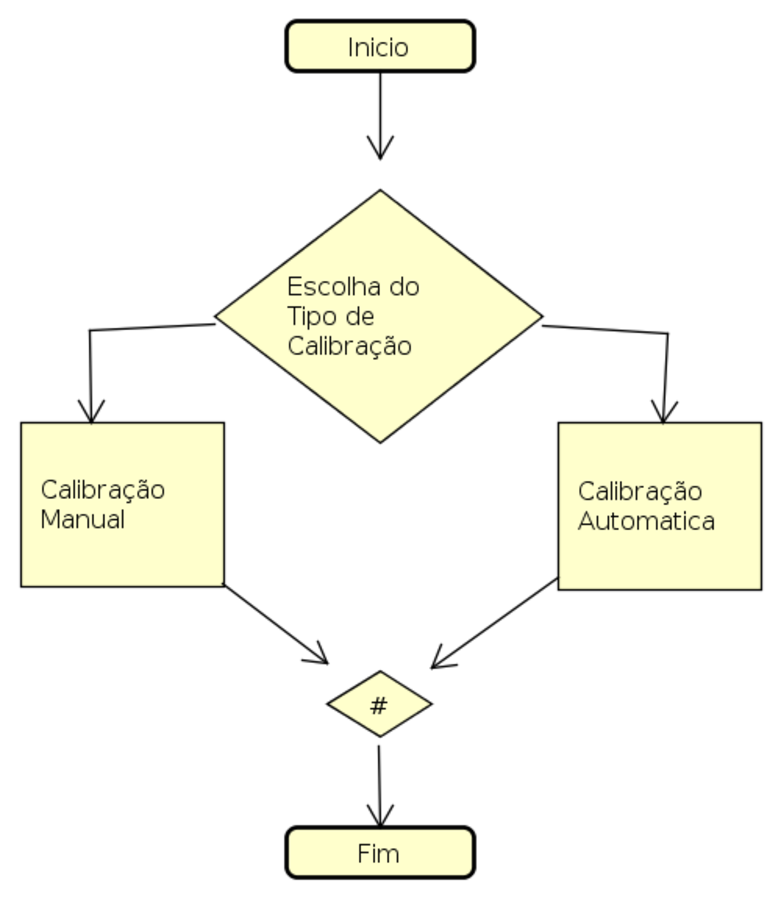
\includegraphics[width=0.45\textwidth]{fluxoprincipal.pdf}
			\caption{Diagrama de Fluxo}
			\label{FlowCHart}
		\end{figure} 
		
		 O fluxo principal do sistema consiste na apresentação da \textbf{interface grafica} ao usuario. A \textbf{interface grafica} por sua vez oferece as duas possibilidades de calibração: Calibração Manual e Calibração Automatica. De acordo com o tipo de calibração escolhido o sistema inicia um subfluxo. Apos a execução de todo subfluxo o sistema é finalizada.
		
	\subsection{Fluxo de Calibração Manual}	
 	O fluxo de calibração manual é iniciado somente se a camera estiver disponivel. Após a camera ser inicializada(1) o sistema espera pela seleção do objeto(2) o qual tera seus pixeis calculados para gerar os valores HSV. Com o objeto selecionado o usuario escolhe entao a cor(4), na opção de escolha de cor, e calibrar. A area selecionada é então analizada e os valores de cada pixel calculados analizando seu HSV(3).
 	O usuario então seleciona os valores que considera satisfatorios(5). Enquanto houverem objetos a serem calibrados(6) o sistema repete esta mesma rotina, quando todos os objetos já tiverem sido calibrados, um arquivo com os valores é gerado(7) e o usuario finaliza o sistema.
		\begin{figure}[!h]
				\centering
				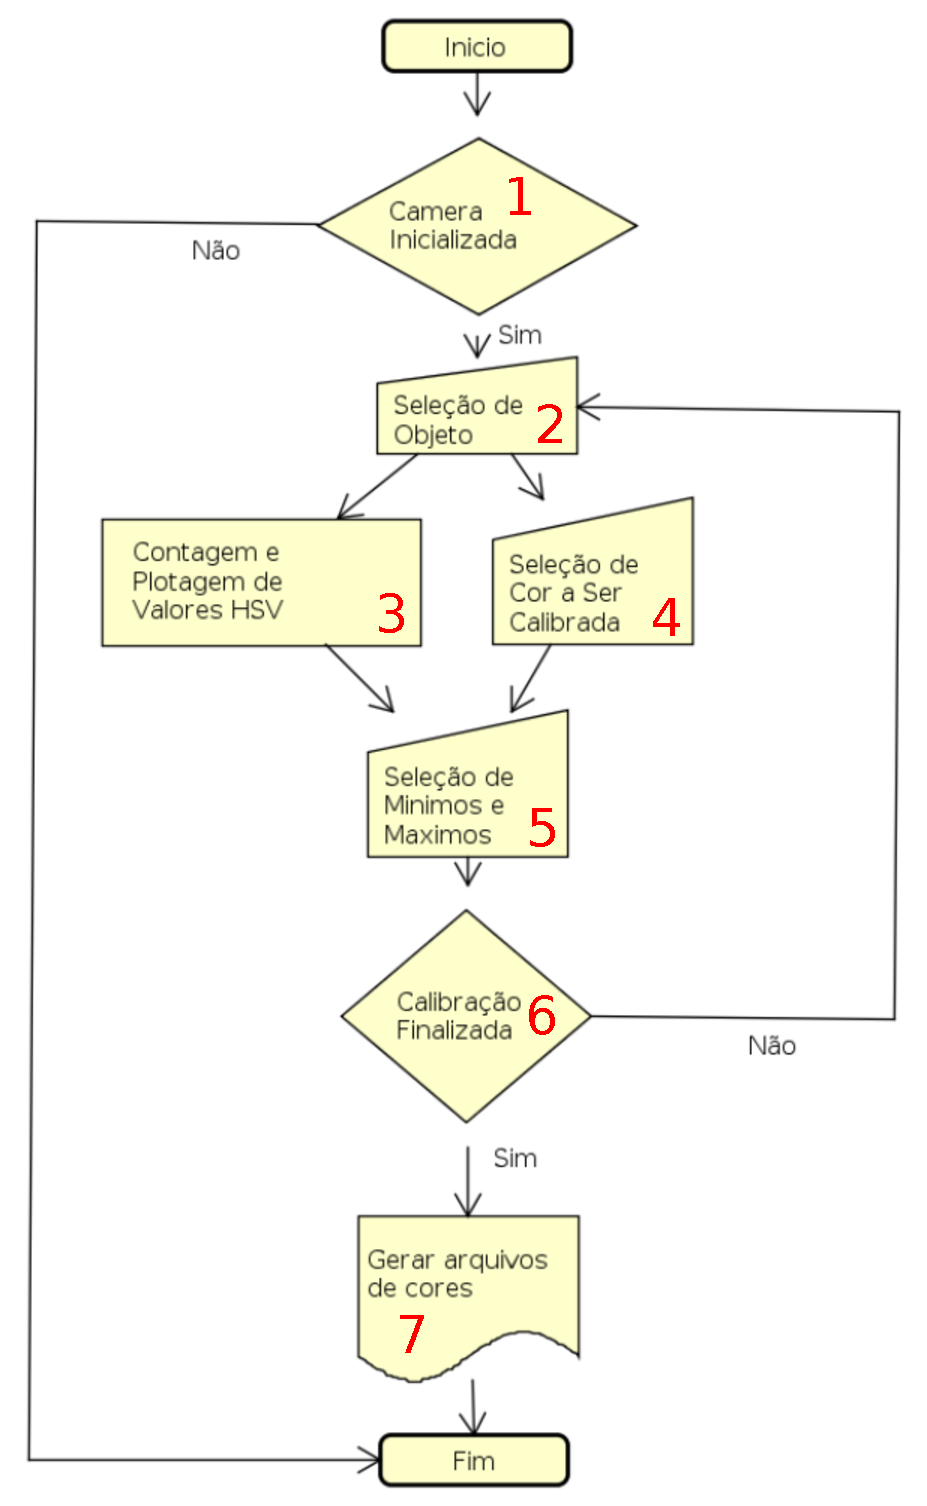
\includegraphics[width=0.45\textwidth]{fluxomanual.pdf}
				\caption{Diagrama de Fluxo Manual}
				\label{DiagramaDeFluxoManual}
			\end{figure}
	\subsection{Fluxo de Calibração Automatica}	
	O fluxo de calibração automatica possui o minimo possivel de interação com o usuario. Neste fluxo o sistema faz automaticamente a detecção de objetos e utilizando a probabilidade matematica conhecida com T de Student verifica o tamanho de cada objeto encontrado para gerar um limite considerado o tamanho que os objetos que devem ser encontrados terão, nesse caso as etiquetas de cores dos robos e só então analizar os valores e calcular os valores minimos e maximos de HSV automaticamente.	
	O fluxo inicia somente caso a camera esteja disponivel(1), apos a sua inicialização é feita a configuração da camera(2), enquadramento do tamanho correto e correção de brilho e luminosidade. Uma vez que a camera está configurada o sistema inicia a deteção de objetos e a validação dos objetos(3) que estão no tamanho correto. Apos deixar somente os objetos corretos no sistema, os pixeis de cada um são varridos e seu intervalo HSV encontrado(4). Os objetos e cores encontrados ficam disponiveis para o usuario apra esse fazer a assimilação entre os objetos e as cores corretas(5), após intervalos corretos já tiverem sido calibrados, um arquivo com os valores é gerado(6) e o usuario finaliza o sistema.
		\begin{figure}[!h]
				\centering
				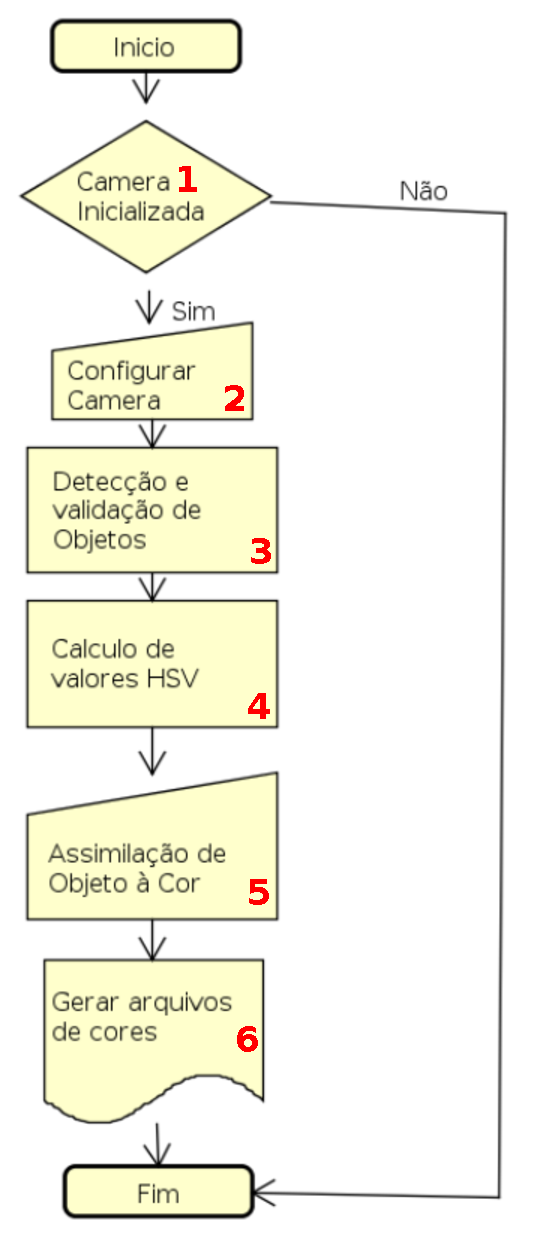
\includegraphics[width=0.45\textwidth]{fluxoautomatico.pdf}
				\caption{Diagrama de Fluxo Automatico}
				\label{DiagramaDeFluxoAutomatico}
			\end{figure} 
			
		Nas sessões à seguir explicarei detalhadamente cada processo da calibração automatica
	\subsubsection{Configuração de Camera}
Antes de ser feito o processo de calibração são necessarias duas configurações: Constrate e Brilho e o Recorte de Imagem.
A configuraça~o de contraste e brilho utiliza o metodo \textit{convertTo} da biblioteca \textit{OpenCV} e é utilizada para o melhoramento da imagem antes da detecção dos objetos, a utilização completa fica da seguinte maneira:
\begin{center}
\centering \textit{ frameA.convertTo(frameA, -1, contrast\_value / 50.0, brightness\_value)}
\end{center}
Esta função recebe quatro parametros. O primeiro \textbf{frameA} informa aonde sera salvo o resultado da conversão. O segundo \textbf{-1} indica o tipo da matrix, ou numero de canais, da imagem a ser gerada, usa-se -1 quando se deseja que se use os valores semelhantes aos da imagem da imagem original\cite{OpenCV}, O terceiro \textbf{contrast\_value / 50.0} indica o valor de constraste, ou alpha, a ser usado para multiplicar os valores do pixel da imagem\cite{OpenCV} e por ultimo \textbf{brightness\_value} que é o valor do brilho, ou beta, a ser adicionado à imagem. \newline
Outra configuração feita é o Recorte de Imagem, onde utilizando a função setMouseCallback para possibilitar a interção do usuario na imagem por meio do mouse, sua utilização é dada da seguinte maneira:
\begin{center}
\centering \textit{ cv::setMouseCallback(src\_window,mouseHandler,0);}
\end{center}
Tem como primeiro parametro \textbf{src\_windows} que indica a janela na qual a função recebera a interação,  o segundo, \textbf{mouseHandler}, indica a função na qual esta implementada a interação e o ultimo parametro, \textbf{0}, indica parametros opcionais, neste caso não usaremos nenhum então foi usado o numero 0.
Dentro da função \textbf{mouseHandler} são identificados os pontos iniciai e final da seleção na tela e utilizada a função \textit{rectangle} para demarcar a seleção na tela. A utilização da função \textit{rectangle} completa fica da seguinte maneira:
\begin{center}
\centering \textit{ cv::rectangle(frameA, point1, point2, CV\_RGB(255, 0, 0), 2, 5, 0);}
\end{center}
A função rebece os parametros \textbf{frameA} indicando a imagem na qual será demarcada a area selecionada, depois o parametro \textbf{point1} que é o ponto incial de seleção na imagem, \textbf{point2} que é o ponto final da seleção. \textbf{CV\_RGB(255, 0, 0)} que indica a cor da demarcaç~ao, \textbf{2} indicando a expessura da demarcação, \textbf{5} que significa o tipo de linha a ser utilizado na demarcação e \textbf{0} que é o numero de bits fracinarios.
 Após confirmada a escolha do tamanho da tela 
este é então salvo na variavel nomeada \textit{tamanho}, está então sera usado durante todo o processo de calibração.
\newpage
\subsubsection{Detecção e validação de Objetos}
A detecção dos objetos a serem calibrados é dada pelo algoritmo de detecção de bordas de Canny. Como mais um recurso para eliminação de ruidos e melhoria da imagem antes de ser executado a detecção de objetos atravez da detecção de bordas é utilizado desfoque na imagem. O algoritmo de Canny já está implementado dentro da biblioteca OpenCV e com a seguite usagem:
\begin{center}
\centering \textit{  Canny(src\_gray, canny\_output, thresh, thresh * 3, 3);}
\end{center}
O algoritmo de Canny utiliza por padrão imagem em padrões de cinza, sendo assim \textbf{src\_gray} é a imagem orignal tranformada para escala de cinza, esta é a imagem na qual o algoritmo sera aplicado. \textbf{canny\_output} será a imagem de saida da função.
\textbf{thresh} e \textbf{thresh*3} são os limites minimos e maximos para considerar uma borda. \textbf{3} é o valor de apertura ou kernel, o valor 3 é utilizado como padro.

Apos o uso do algoritmo de Canny para detecção de bordas é necessario então fazer uso da função \textit{findContours}, nativa no \textit{OpenCV} para detecção de contornos.
\begin{center}
\centering \textit{ findContours(canny\_output, contours, hierarchy, CV\_RETR\_EXTERNAL, CV\_CHAIN\_APPROX\_SIMPLE, Point(0, 0))}
\end{center}

O primeiro parametro, \textbf{canny\_output}, é a imagem que o algoritmo de Canny gerou com as bordas encontrada na imagem, e é a imagem que o método \textit{findContours} ira utilizar para detectar os contornos, \textbf{contours} é o parametro que indica onde serão salvos os contornos encontrados, cada contorno é armazenado como sendo um vetor de pontos \cite{OpenCV}. \textbf{hierarchy} é onde será salva um verot de informações sobre a topologia da imagem, e terá como total de elementos o mesmo numero que o total de contornos encontrado\cite{OpenCV}. O quarto parametro, \textbf{CV\_RETR\_EXTERNAL} indica o modo de obtenção de contornos, nesse caso \textit{CV\_RETR\_EXTERNAL} indica que o metodo só obtera os contornos exteriores\cite{OpenCV}. \textbf{CV\_CHAIN\_APPROX\_SIMPLE} indica o metodo que sera usado para aproximaç~ao de contornos, o metodo \textit{CV\_CHAIN\_APPROX\_SIMPLE} comprime segmentos horizontais, verticais, diagonais e deixa apenas os seus pontos finais\cite{OpenCV}. E o ultimo parametro, \textbf{Point(0, 0)}, indica o valor a ser usado para deslocar a imagem ao encontrar os objetos, neste caso esse valor é 0 para Y e 0 para X, pois não sera necessario. 

Uma vez obtidos os contornos é necessarios que se faça a eliminação de vertices dos polignos encontrados nos objetos deixando assim o objeto mais preciso. Isso é necessario para deixar a forma encontrada mais precisa dá forma original. Para este ajuste foi usado o metodo \textit{approxPolyDP}, ja implementado dentro da biblioteca OpenCV. Esse metodo teve que ser aplicado em cada um dos contornos encontrados, e foi utilizado da seguinte maneira:
\begin{center}
\centering \textit{    approxPolyDP(Mat(contours[i]), contours\_poly[i], 3, true)}
\end{center}
 Onde o metodo inicia recebendo como paralametro, \textbf{Mat(contours[i])} que é a criação de uma nova imagem, somente com aquele unico objeto, que esta sendo analisado. A seguir é informado no segundo parametro a variavel de destino \textbf{contours\_poly[i]}, onde sera salvo o objeto com a eliminação dos vertices. O terceiro parametro indica o valor do \textit{epilson}, usado o valor \textbf{3} que especifica a precisão da aproximação, a distância máxima entre a curva original e a sua aproximação\cite{OpenCV}. O ultimo parametro indica se a curva aparoximada sera fechada ou não, foi usado o valor \textbf{true} pois neste caso fechar um uma curva é necessario para que o objeto onde está a cor, seja idenficado e analizado na probabilidade.
 
 Por ultimo os objetos possuem sua borda ignorada, sendo assim calculado o tamanho interior dele, para que por ventura não hajam pixeis de cor preta ou derivadas a serem calculadas.
 
 A detecção de contorno detecta todos os contornos possiveis na imagem, isso inclue sombras, luzes entre outras coisas. Mas nao são todos os objetos encontrados que deverão ser calculados, sendo assim foi usado o calculo probabilistico T de Student.
 Foi implementado uma biblioteca para o uso da probabilidade voltada para objetos Rect, os objetos da biblioteca \textbf{OpenCV} obtidos na detecção. Essa biblioteca analiza a lista de objetos encontrados na detecção e faz o calculo dos limites, tamanho minimo e maximo, dos objetos. Apos a obtenção desse limite pela biblioteca são analizados todos os objetos encontrados na detecção e os cujo tamanho não esteja dentro deste limite são removidos da lista.
 \newpage
 \subsubsection{Calculo de valores HSV}
 

